\documentclass[12pt]{article}

\usepackage[utf8]{inputenc}
\usepackage[a4paper, total={6in, 10in}]{geometry}

\title{Linear Time Sorting}
\author{Manuel Serna-Aguilera}
\date{}
\setlength{\parindent}{0pt}

\usepackage{natbib}
\usepackage{graphicx}
\usepackage{amsmath}
\usepackage{clrscode3e}

\begin{document}

\maketitle

\section*{Introduction}
We have looked at sorting algorithms that sort $n$ elements in $O(n \cdot \log_2{(n))}$ time, these were all comparison sorts, meaning all they do to gather information on data to be sorted is to compare elements. The best any comparison sorting algorithm can do is $\Omega(n \cdot \log_2{(n))}$, with merge sort and heapsort being asymptotically optimal comparison sorts. We can actually sort elements in less time than this, but in doing so (at least in the algorithms the book covers) we will need to tack on an assumption in our analysis. We shall look at three sorting algorithms that do no need to compare to sort, and thus the $\Omega(n \cdot \log_2{(n))}$ time does not apply to them.

\section*{Counting Sort}
Counting sort assumes that each of the $n$ input elements is an integer in the range 0 to $k$,  for some integer k.
\\ \\
This sorting algorithm determines, for each input element $x$ , the number of elements less than $x$. We then place $x$ after that many elements in the output array. As an example, if there are 17 elements less than $x$, then $x$ would be in output position 18; we would have to account for duplicate elements, but this is the general idea.
\\ \\
In the pseudocode below, assume the input is an array $A[1 \twodots n]$, and thus $\attrib{A}{length} = n$. There are two other arrays used: $B[1 \twodots n]$ contains the sorted output,  while the array $C[0 \twodots k]$ provides temporary working storage.

\clearpage

\begin{figure}[!ht]
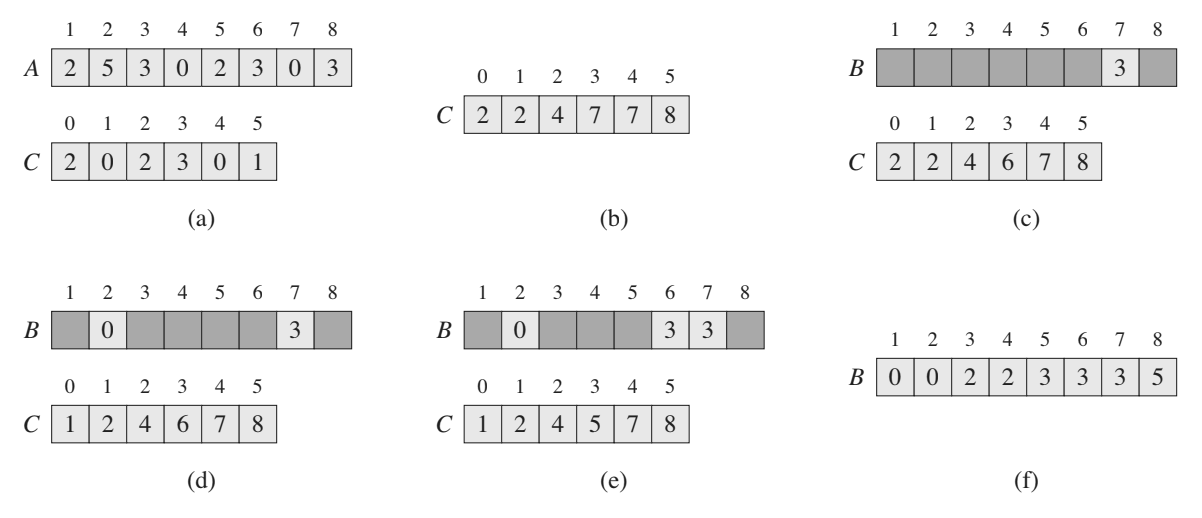
\includegraphics[scale=0.45]{counting_sort}
\caption{
    Calling $\proc{counting-sort}$ on input array $A[1 \twodots 8]$, where each integer is nonnegative and no larger than $k=5$.
    \textbf{(a)} Arrays $A$ and $C$ after line 5. Each index $i$ in $C$ now holds how many times each integer appears in $A$. 
    \textbf{(b)} $C$ after line 8.
    \textbf{(c)-(e)} The output array B after three iterations in the loop from lines 10-12.
    \textbf{(f)} The final sorted array B.
}
\label{fig:linear_cs}
\end{figure}

%------------------------------------------------
% Counting sort
%------------------------------------------------
\begin{codebox}
\Procname{\proc{counting-sort}$(A, B, k)$}
\li let $C[0 \twodots k]$ be a new array
\li \For $i \gets 0$ \To $k$
\li \Do 
        $C[i] = 0$ \Comment initialize
    \End
\li \For $j \gets 1$ \To $\attrib{A}{length}$
\li \Do
        $C[A[j]] = C[A[j]] + 1$
    \End
\li \Comment $C[i]$ now contains the number of elements equal to $i$
\li \For $i \gets 1$ \To $k$
\li \Do
        $C[i] = C[i] + C[i-1]$
    \End
\li \Comment $C[i]$ now contains the number of elements less than or equal to $i$
\li \For $j \gets \attrib{A}{length}$ \Downto $1$
\li \Do
        $B[C[A[j]]] = A[j]$
\li    $C[A[j]] = C[A[j]] - 1$
    \End
\end{codebox}

Breaking the running time down, lines 2-3 and 7-8 take $\Theta{(k)}$ time, while lines 4-5 and 10-12 take $\Theta{(n)}$ time, the running time for counting sort is $\Theta{(n + k)}$; in practice this algorithm is used when $k = O(n)$, in which case the running time is $\Theta{(n)}$.
\\ \\
An important property of counting sort is that it is \textbf{stable}, meaning numbers with the same value appear in the output array in the same order as in the input array. For example, if you have three twos, $2_1, 2_2, 2_3$, counting sort should \textbf{not} produce a different ordering in $B$, the order should still be $\ldots, 2_1, 2_2, 2_3, \ldots$.

\newpage

\section*{Radix Sort}
Radix sort operates on integers, and its assumption is that these integers have $d$ digits. It starts by sorting the \textit{least significant} digit first, and then moves up, sorting increasingly significant digits along the way, to sort digit $d$. After only $d$ passes, we end up with sorted numbers. For radix sort to work correctly, the digit sort must be \textit{stable}.

\begin{figure}[!ht]
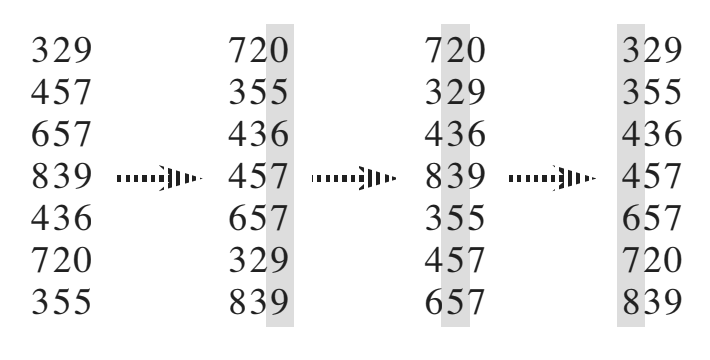
\includegraphics[scale=0.4]{radix_sort}
\caption{
    The operation of radix sort on a list of seven 3-digit numbers. The input is taken at the left, the least-significant digit is sorted first (shading indicates what digit is being sorted), then the second, and then the last digit $d=3$. The result is a list of sorted numbers.
}
\label{fig:linear_rs}
\end{figure}

An example of applying radix sort would be sorting records by day first, then month, and then year. The pseudocode for radix sort is just a for loop iterating on each digit, the real meat is the sorting algorithm used to sort the digits. Something like counting sort would do just fine, since we know it is stable. This procedure assumes the $n$-element array $A$ has $d$ digits, where digit 1 is the least significant and $d$ the most significant.

%------------------------------------------------
% Radix sort
%------------------------------------------------
\begin{codebox}
\Procname{\proc{radix-sort}$(A, d)$}
\li \For $i \gets 1$ to $d$
\li \Do
        use a stable sort to sort array $A$ on digit $i$
    \End
\end{codebox}

\textbf{Lemma} \\
Given $n$ $d$-digit numbers in which each digit can take on up to $k$ possible values, $\proc{radix-sort}$ correctly sorts these numbers in $\Theta{(d(n + k))}$ time if the stable sort it uses takes $\Theta{(n + k)}$.
\\ \\
Recall what all those values were:\\
\begin{itemize}
    \item[] $d=$ number of digits,
    \item[] $n=$ length of list,
    \item[] $k=$ possible values.
\end{itemize}


\newpage

\section*{Bucket Sort}
Bucket sort assumes that the input is drawn from a uniform distribution and has an average-case running time of $O(n)$. Specifically, the assumption is that the input is generated by a random process that distributes elements uniformly and independently over the interval $[0, 1)$. Bucket sort basically divides this uniformly distributed input into $n$ equally-sized subintervals, or buckets, and distributes the values into the buckets. We then sort the smaller buckets and overall we have a sorted output array $B$ as in figure 3.

\begin{figure}[!ht]
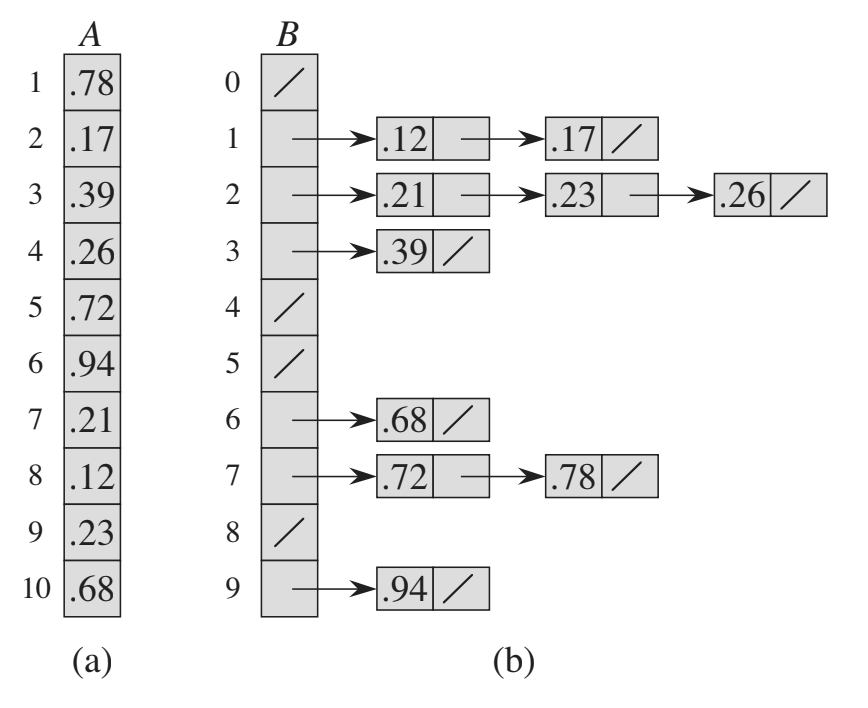
\includegraphics[scale=0.3]{bucket_sort}
\caption{
    The operation of $\proc{bucket-sort}$ for $n=10$. 
    \textbf{(a)} The input array $A[1 \twodots 10]$.
    \textbf{(b)} The array $B$ with sorted buckets after line 8. Bucket $i$ holds values in the half-open interval $[i/10, (i+1)/10)$.
}
\label{fig:linear_bs}
\end{figure}

%------------------------------------------------
% Bucket sort
%------------------------------------------------
\begin{codebox}
\Procname{\proc{bucket-sort}$(A)$}
\li $n \gets \attrib{A}{length}$
\li let $B[0 \twodots n-1]$ be a new array
\li \For $i \gets 0$ to $n-1$
\li     \Do
            make $B[i]$ an empty list
        \End
\li \For $i \gets 1$ to $n$
\li     \Do
            insert A[i] into list $B[\lfloor n A[i] \rfloor]$
        \End 
\li \For $i \gets 0$ to $n-1$
\li     \Do
            sort list $B[i]$ with insertion sort
        \End
\li concatenate the lists $B[0], B[1], \ldots, B[n-1]$ together in order
\end{codebox}

With this procedure, the worst-case running time of bucket sort would be $\Theta(n^{2})$. If the assumption is broken, and if we have all our values in one bucket and in reverse order, then insertion sort would take $\Theta(n^{2})$ time. To not invoke the $\Theta{(n^2)}$ running time, use heapsort instead, which is asymptotically optimal with its worst-case running time being $O(\log_2(n))$.

\end{document}
